\subsubsection{Bestimmen und Fitten der Peaks}
\label{sec:peaks}
In diesem Versuchsteil wurde ein Pulverdiffaktogramm von Kochsalz (NaCl) aufgenommen. Das rohe so aufgenommene Spektrum ist in Abb.~\ref{fig:rohspektrum} dargestellt.
\begin{figure}[h!]
    \centering
    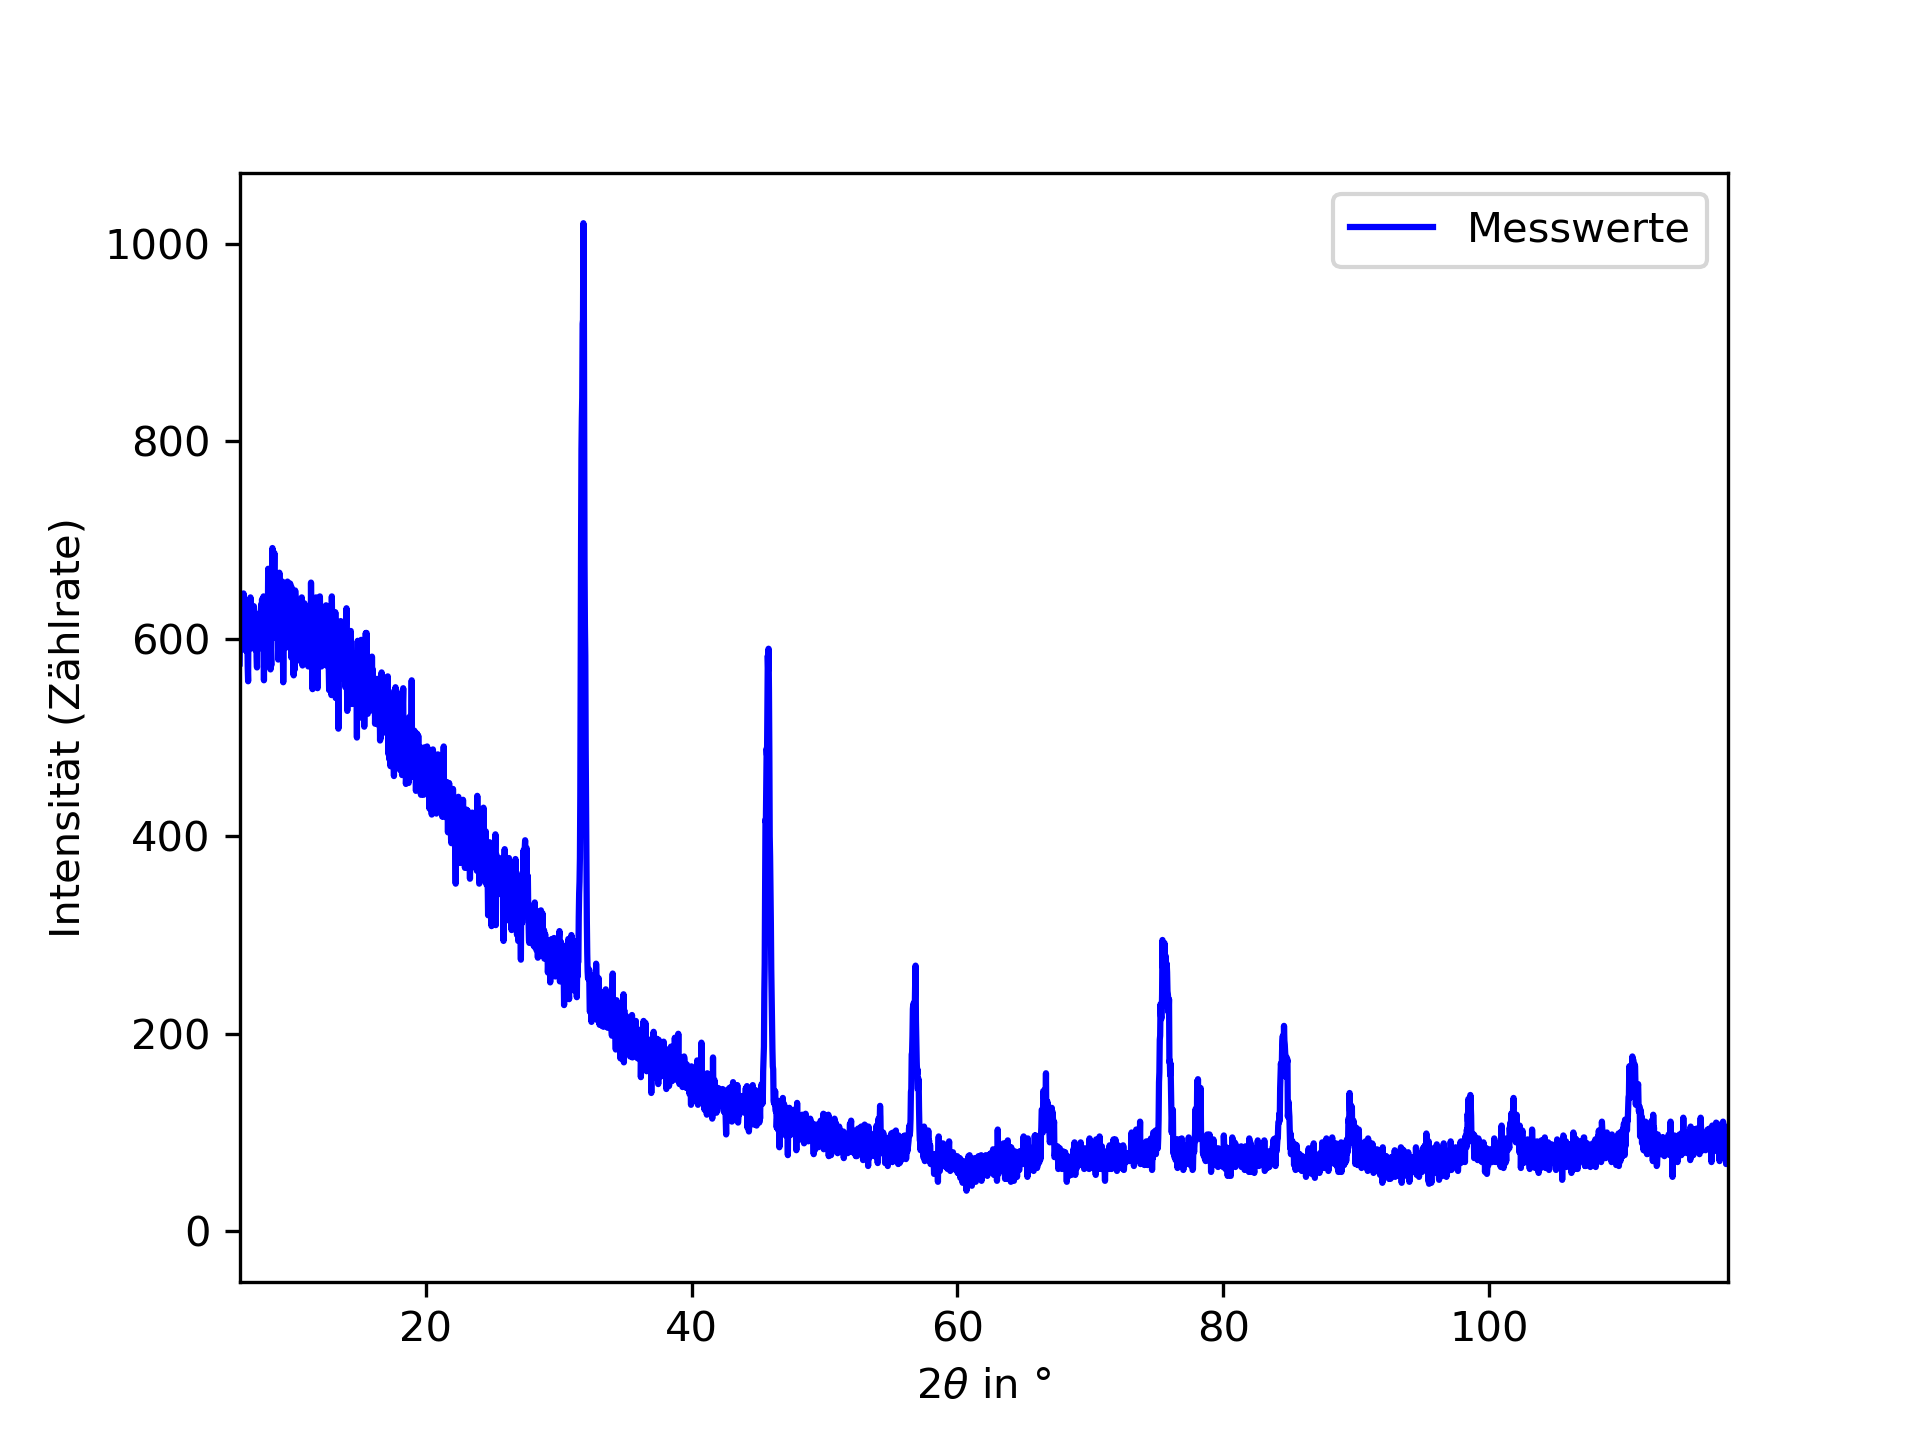
\includegraphics[width=0.7\textwidth]{spektrum_roh.png}
    \caption{Aufgenommenes Diffkaktogramm von Kochsalz mit der Zählrate $I$ gegen den Streuwinkel $2\Theta$.}
    \label{fig:rohspektrum}
\end{figure}

Die so aufgenommenen Daten sollen nun insbesondere anhand der Peaks analysiert werden. 
Um insbesondere die kleinen Peaks besser zu finden, wird das Spektrum zunächst mit einem Savitzky-Golay-Filter geglättet. Die so geglätteten Daten sind in Abb.~\ref{fig:geglättet} dargestellt, in der die Peaks bereits indiziert sind.
\begin{figure}
    \centering
    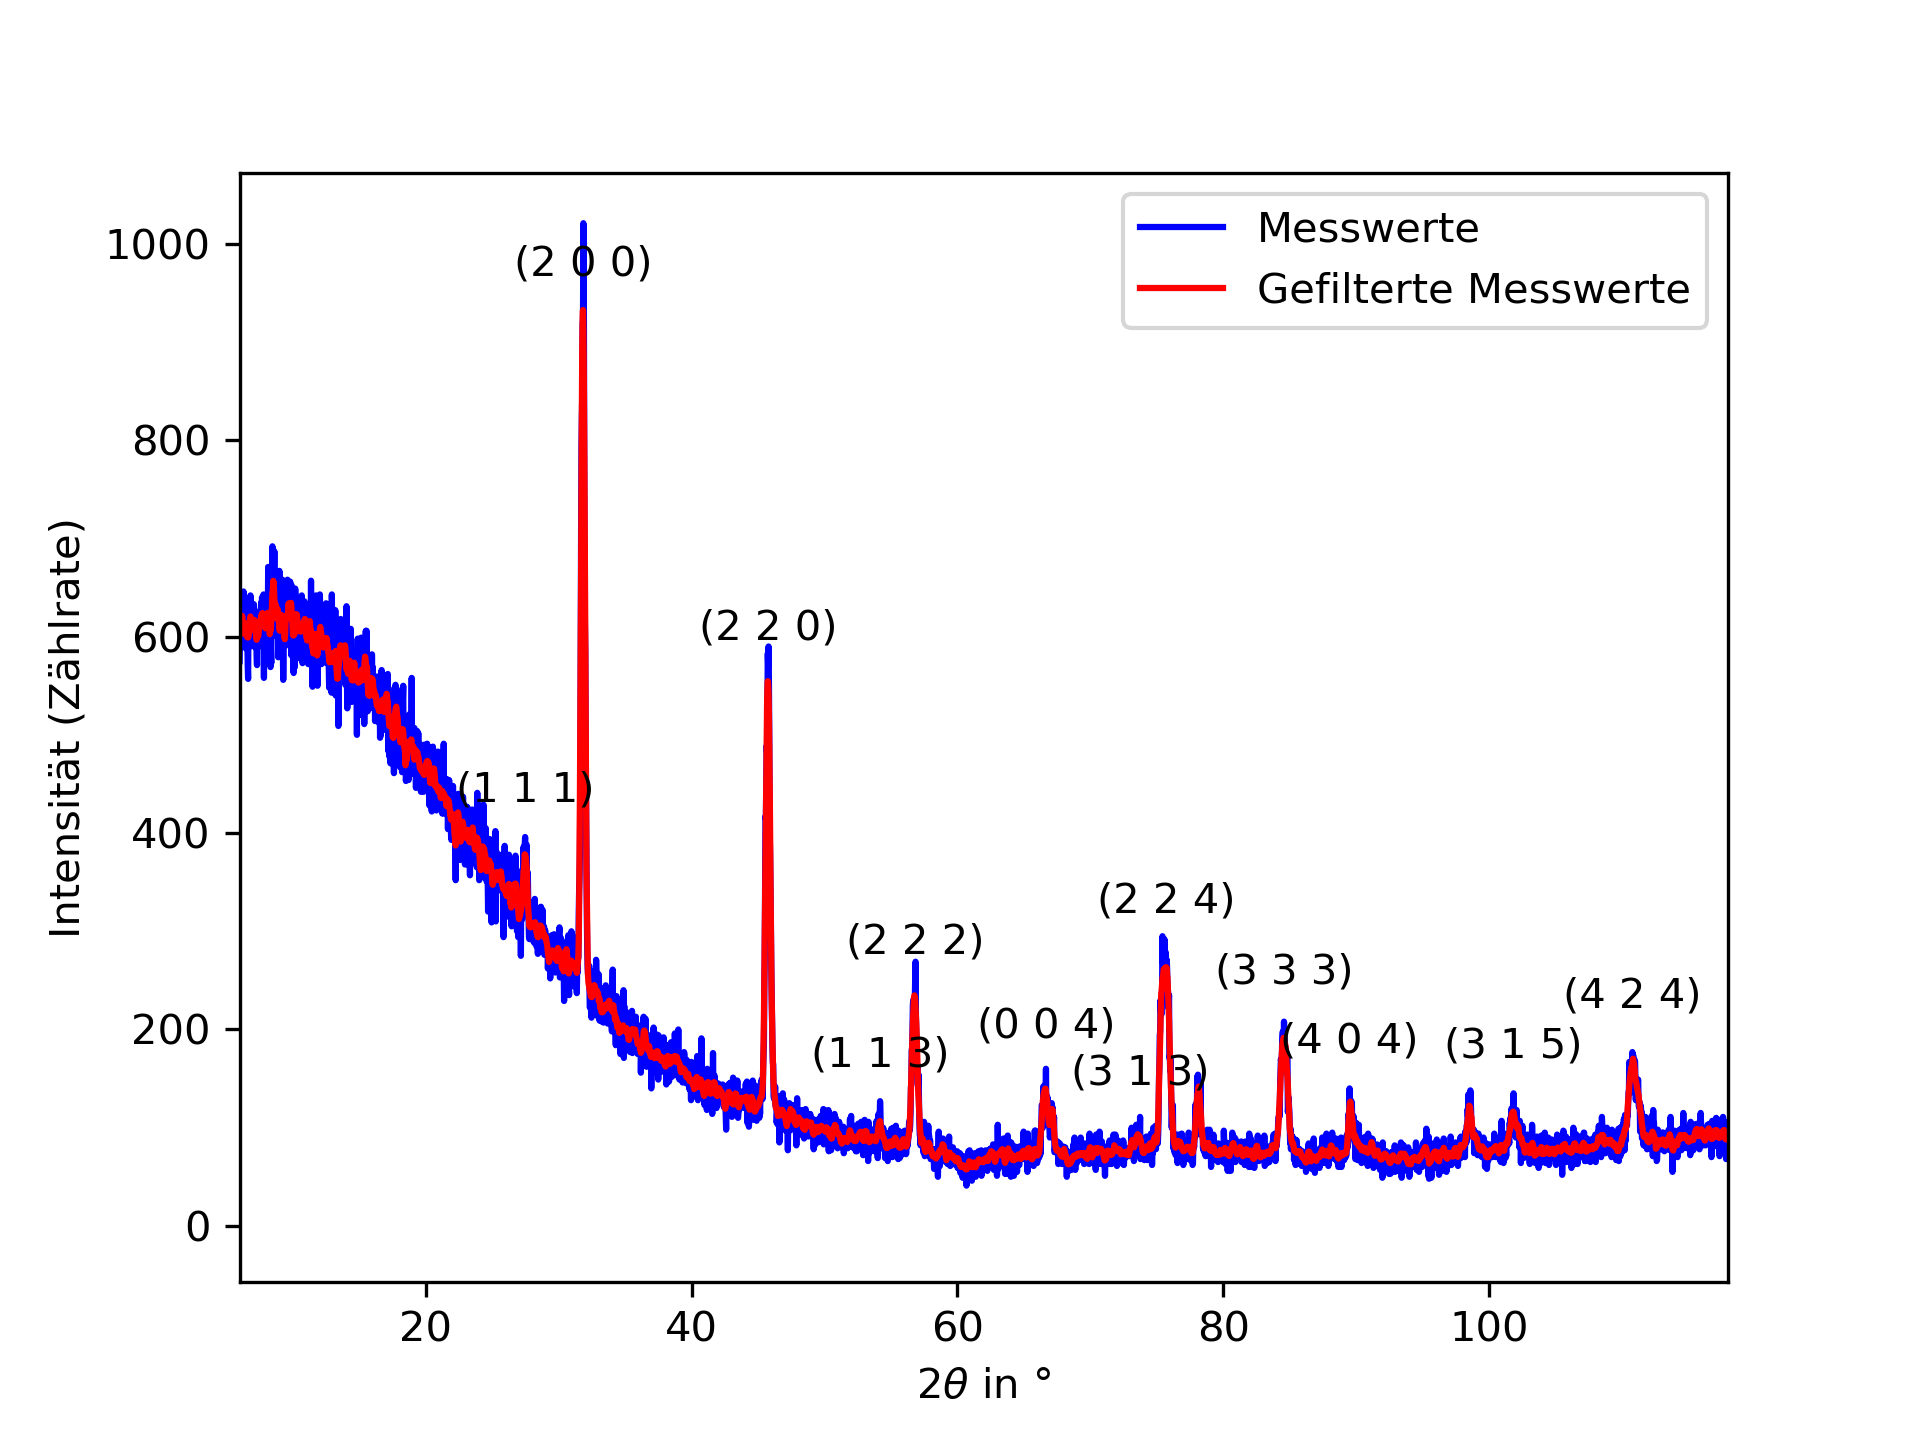
\includegraphics[width=0.7\textwidth]{indiziert.png}
    \caption{Gefiltertes Spektrum von Kochsalz mit der Zählrate $I$ gegen den Streuwinkel $2\Theta$. Das rohe Spektrum ist in blau, das geglättete in rot dargestellt. Ebenso sind die Peaks mit ihren Millerschen Indizes beschriftet.}
    \label{fig:geglättet}
\end{figure}
Mithilfe der Software Jana2020 \footnote[1]{Institute of Physics,Department of StructureAnalysis, Cukrovarnicka 10, 16253 Praha 6, Czech Republic} wird nun probiert, die Peaks mit einer Pseudo-Voigt-Funktion zu fitten. Als Anfangsfitwert für den Gitterparameter wird hierbei der Literaturwert $a = \SI{5,64}[]{\angstrom}$ verwendet. Peaknummer, händisch bestimme Peaklage $2\theta_{[Auge]}$, gefittet Peaklage $2\theta_{[Fit]}$ sowie die Halbwertsbreite sind in Tabelle~\ref{tab:peaks} dargestellt.


\begin{table}[h!]
    \centering
     \begin{tabular}{|c|c|c|c|} 
     \hline
     Peak-Nr. & $2\theta_{[Auge]}$ in ° & $2\theta_{[Fit]}$ in ° & FWHM in ° \\ [0.5ex] 
     \hline\hline
     1 & \num{27,46(0,05)} & \num{27,518(0,005)} & \num{0,308(0,005)} \\ 
     2 & \num{31,85(0,03)} & \num{31,881(0,005)} & \num{0,311(0,005)} \\
     3 & \num{45,78(0,05)} & \num{45,709(0,005)} & \num{0,324(0,005)} \\
     4 & \num{54,18(0,03)} & / & / \\
     5 & \num{56,85(0,03)} & \num{56,808(0,005)} & \num{0,338(0,005)} \\ 
     6 & \num{66,66(0,03)} & \num{66,634(0,005)} & \num{0,355(0,005)} \\
     7 & \num{73,75(0,05)} & / & / \\
     8 & \num{75,43(0,03)} & \num{75,774(0,005)} & \num{0,375(0,005)} \\
     9 & \num{84,58(0,03)} & \num{84,554(0,005)} & \num{0,399(0,005)} \\
     10 & \num{89,52(0,05)} & / & / \\
     11 & \num{101,86(0,03)} & \num{101,934(0,005)} & \num{0,467(0,005)} \\
     12 & \num{108,51(0,05)} & / & / \\
     13 & \num{110,80(0,03)} & \num{110,955(0,005)} & \num{0,517(0,005)} \\  [1ex] 
     \hline
     \end{tabular}
     \caption[short]{Tabelle der Peaks mit händisch bestimmten Werten und gefitteten Werten sowie der Halbwertsbreite der gefitteten Peaks.}
     \label{tab:peaks}
\end{table}

Hierbei wird ersichtlich, dass nicht für alle Peaks ein sinnvoller Fit möglich war. Ebenso war die integrierte Intensität mit der Software nicht möglich und auch ansonsten sehr komplex und aufwändig. Daher wird hier auf eine Diskussion der Intensitäten verzichtet.

\subsubsection{Gitterparameter und Diskussion}

Nun soll für jeden erfolgreich gefitteten Peak der zugehörige Netzabstand berechnet werden. Hierbei gilt unter Annahme eines kubischen Kristallgitters:
\begin{equation}\label{eq:netzabstand}
    \frac{1}{d^2_{hkl}} = \frac{h^2 + k^2 + l^2}{a^2}
\end{equation}
mit $h, k, l$ den Millerschen Indizes und $a$ dem Gitterparameter. Mithilfe der Braggschen Beugungsbedingung
\begin{equation}
    2d\sin(\theta) = n\lambda
\end{equation}

mit $n = 1$ der Beugungsordnung und $\lambda = \SI{1,5406}{\angstrom}$ der Wellenlänge der Röntgenstrahlung, kann der Gitterparameter berechnet werden:

\begin{equation}
    \sin^2(\theta) = \frac{\lambda^2}{4a^2} \cdot (h^2 + k^2 + l^2)
\end{equation}

Die Ergebnisse für den Netzabstand $d_{hkl}$, deren quadrierten Sinus des Beugungswinkels, die Konstante $\nicefrac[]{\lambda^2}{4a^2}$ und den Gitterparameter $a$ sind in Tabelle~\ref{tab:gitter} dargestellt. Ebenso werden die Millerschen Indizes für den jeweiligen Peak angegeben.

\begin{table}[h!]
    \centering
     \begin{tabular}{|c|c|c|c|c|c|c|c|} 
     \hline
     Peak-Nr. & $2\theta_{[Fit]}$ & $d/\si{\angstrom}$ & $\sin^2(\theta)$ & $\frac{\lambda^2}{4a^2}$ & $(h^2+k^2+l^2)$ & $a/\si{\angstrom}$ &  $h k l $ \\ [0.5ex] 
     \hline\hline
     1 & \num{27,518(0,005)} & 3,2387 & 0,056568 & 0,018856 & 3 & 5,6096 & 1 1 1 \\
     2 & \num{31,881(0,005)} & 2,8048 & 0,075424 & 0,018856 & 4 & 5,6096 & 2 0 0 \\
     3 & \num{45,709(0,005)} & 1.9833 & 0.150849 & 0,018856 & 8 & 5,6096 & 2 2 0 \\
     5 & \num{56,808(0,005)} & 1.6194 & 0.226273 & 0,018856 & 12 & 5,6096 & 2 2 2 \\ 
     6 & \num{66,634(0,005)} & 1.4024 & 0.301698 & 0,018856 & 16 &  5,6096 & 0 0 4\\
     8 & \num{75,774(0,005)} & 1.2543 & 0.377122 & 0,018856 & 20 &  5,6096 & 2 0 4\\
     9 & \num{84,554(0,005)} & 1.1451  &  0.452546 & 0,018856 & 24 &  5,6096 & 2 2 4\\
     11 & \num{101,934(0,005)} & 0.9916 & 0.603395 & 0,018856 & 32 &  5,6096 & 4 0 4\\
     13 & \num{110,955(0,005)} & 0.9349 & 0.678820 & 0,018856 & 36 &  5,6096 & 4 2 4\\ [1ex] 
     \hline
     \end{tabular}
     \caption[short]{Tabelle mit den berechneten Werten für den Netzabstand $d_{hkl}$, dem quadrierten Sinus des Beugungswinkels des jeweiligen Peaks, der Konstante $\nicefrac[]{\lambda^2}{4a^2}$ und dem Gitterparameter $a$. Ebenso werden die Millerschen Indizes für den jeweiligen Peak angegeben. In der Tabelle sind nur die Peaks, für die ein Fit möglichm war.}
     \label{tab:gitter}
\end{table}

Wie man sieht, ist der Gitterparameter $a$ für alle Peaks gleich. Dies liegt natürlich auch an der Natur des Fits, welcher den Gitterparamter berechnet, für den die Abweichungen der gemessenen Werte von den theoretisch bewerteten Werten minimal sind. Daher ist die Mittelwertbildung hier überflüssig, eher kann man direkt den berechneten Wert für $a$ nehmen, den Jana2020 berechnet. Hiermit ergibt sich:

\begin{equation}
    a = \SI{5,6096(0,0005)}{\angstrom}
\end{equation}

Dies ist nah am Literaturwert von $a = \SI[]{5,6418}[]{\angstrom}$~\cite{fon}, was für die Qualität des Fits und auch der Messung spricht. Nichtsdestotrotz ist der Wert nicht perfekt. Dies kann an systematischen Fehlern in der Messung, wie beispielsweise der Eichung des Detektors, liegen. Ebenso kann es sein, dass die Probe nicht ideal pulverisiert war, was zu einer Verbreiterung der Peaks führen würde.

Damit können nun auch die Netzabstände mithilfe Gl.~\ref{eq:netzabstand} für die Peaks berechnet werden, bei denen kein Fit möglich war. Die Ergebnisse hierfür sind in Tabelle~\ref{tab:gitter2} dargestellt.

\begin{table}[h!]
    \centering
     \begin{tabular}{|c|c|c|c|c|c|} 
     \hline
     Peak-Nr. & $2\theta_{[Auge]}$ & $d/\si{\angstrom}$ & $\sin^2(\theta)$ & $(h^2+k^2+l^2)$&  $h k l $ \\ [0.5ex] 
     \hline\hline
     4 & \num{54,18(0,03)} & 1.6914 & 0.207380 & 11 & 1 1 3 \\
     7 & \num{73,75(0,05)} & 1.2869 & 0.360085 & 19 & 3 1 3\\
     10 & \num{89,52(0,05)}  & 1.0796 & 0.495811 & 27 & 3 3 3 \\
     12 & \num{108,51(0,05)} & 0.9482 & 0.658735 & 35 & 3 1 5 \\
     [1ex] 
     \hline
     \end{tabular}
     \caption[short]{Tabelle mit den berechneten Werten für den Netzabstand $d_{hkl}$, dem quadrierten Sinus des Beugungswinkels des jeweiligen Peaks und den Millerschen Indizes für die Peaks, für die kein Fit möglich war.}
     \label{tab:gitter2}
\end{table}